\chapter{Fazit}
\section{Auftrag des Projektes}
\section{Kritische Reflexion der Ergebnisse}
\section{Implikationen für Theorie und Praxis}
\section{Ausblick}
% Bevor eine Analyse der Risiken durchgeführt werden kann, müssen zunächst die Terminologie und die Ziele der Durchführung näher dargelegt werden. 
% Für die Definition des Risikos wird die engere Definition des Risikos aus dem Fachbuch „IT-Risikomanagement mit System“ von Hans-Peter Königs verwendet. 
% Die engere Definition des Risikos umfasst eine Abweichung von einem vorher definierten Ziel.
% \footcite[Vgl.][12]{koenigsITRisikomanagementMitSystem2017}
% Bei einem Projekt ist das Ziel der erfolgreiche Abschluss des Projekts.
% Gegenübergestellt kann es Abweichungen in Dauer, Budget und Qualität geben, die den Erfolg des Projekts negativ beeinflussen.
% \footcite[Vgl.][13]{koenigsITRisikomanagementMitSystem2017}
% Die Evidenz für die kritische Relevanz der Risikoabschätzung im Projektkontext führt zu einer großen
% Menge an wissenschaftlichen und unternehmerischen Quellen, die sich mit dem Risiko-Management beschäftigen.
% Das Versagen der Verantwortlichen im Umgang mit Risiken führt zu zahlreichen Möglichkeiten für kontraproduktive Ausgänge für das Projekt und im schlimmsten Fall für das Projektumfeld.
% Ein Beispiel für das Scheitern der Handhabung von Risiken lässt sich im Finanzbereich finden.
% Dort arbeiteten viele Akteure wiederkehrend nicht anforderungskonform, was schließlich in der Finanzkriese 2008 resutlierte.
% \footcite[Vgl.][39]{stulzRiskManagementFailures2008}
% Die hauptsächlichen Fehler, die sich als kritisch erwiesen haben, sind die Fehleinschätzung von Risiken,
% vernachlässigte, ignorierte oder unbekannte Risiken, fehlende Kommunikation und Intransparenz in der Darstellung und Steuerung von Risiken.
% \footcite[Vgl.][S. 42 ff.]{stulzRiskManagementFailures2008}
% Damit diese Fehler vermindert auftreten, beschäftigen sich wissenschaftliche Quellen mit dem Management von Risiken,
% um in der Praxis Möglichkeiten für Bewerkstellligung von Kalkulation, Prognose und mögliche Interventionen umsetzen zu können.
% In der Projektkonzeption und der Einleitung zur Risikoplanung ist es daher essenziell, diese Erkenntnisse zu berücksichtigen
% und ein umfassendes Risikomanagement zu implementieren. Dabei kann ein Projekt in sechs Risikomanagement-Phasen kontinuierlich begleitet werden.
% \footcite[Vgl.][45]{dikmenLearningRisksTool2008}
% In der ersten Phase werden Risiken identifiziert, indem Risikoinformationen und Unsicherheiten zusammengetragen und dokumentiert werden.
% In der zweiten Phase wird eine Bewertung der Risiken durchgeführt, um diese in der dritten Phase angemessen handhaben zu können.
% Diese ersten drei Phasen können innerhalb der Projektkonzeption bereits durchgeführt werden.
% Während der Projektdurchführung werden iterativ die Phasen vier und fünf durchgeführt. Die vierte
% Phase beschäftigt sich mit der Überwachung von Risiken und die fünfte Phase mit den Interventionen im
% Umgang mit Risiken, falls diese eintreten oder sich die Einschätzung ändert. Am Ende eines Projekts
% sollte in einer letzten Phase eine Evaluation des Risikomanagements stattfinden.

% Ergänzend zu diesen Phasen des Risikomanagements existieren Maßnahmen, um auf die einzelnen Risiken zu reagieren.
% \footcite[Vgl.][S. 22 f.]{brandstaeterAgileITProjekteErfolgreich2013}
% Diese Maßnahmen lassen sich aufschlüsseln in Maßnahmen, die präventiver Natur sind, sowie in solche, die erst beim Eintreten
% eines Risikos ausgelöst werden, um die Risikoauswirkungen einzudämmen.
% Ein Beispiel für den Unterschied dieser Maßnahmen ist der Umgang mit Bränden in Gebäuden.
% In vielen Gebäuden ist das Rauchen und Erzeugen eines offenen Feuers verboten, um präventiv zu verhindern, dass ein Brand ausbricht.
% Allerdings werden zur Bekämpfung eines Feuers zusätzlich Feuerlöscher für den Fall bereitgestellt, dass ein Brand ausbrechen sollte.
% Eine Unterscheidung dieser Maßnahmentypen für eine Risikoanalyse kann Mehrwert schaffen, um die reale Gefahr darstellen zu können.
% In der ersten Risikomanagementphase (Risikoidentifikationsphase) werden die Hauptrisiken des Scrum-Verfahrens
% als Leitrisikotypen verwendet\footcite[Vgl.][40]{brandstaeterAgileITProjekteErfolgreich2013}: 
% \begin{figure}[H]
%     \centering
%     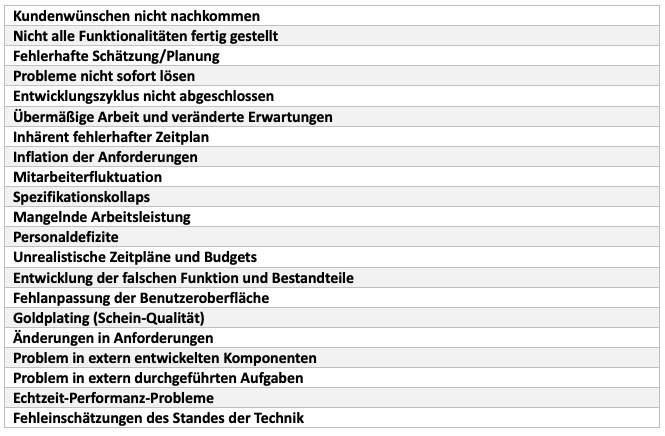
\includegraphics[width=1\linewidth]{graphics/leitrisiko.png}
%     \caption{Übersicht der Leitrisikotypen.}\label{abb:zeitplanung}
% \end{figure}
% Anhand dieser Hauptrisiken werden potenzielle Probleme und Herausforderungen für das bestehende Projekt abgeleitet.
% Ebenso werden zur Vermeidung und Bewerkstelligung von Risiken präventive und reaktive Maßnahmen erarbeitet, welchen
% als Leitbild ein entsprechendes Risikoregister zugrunde liegt.
